\documentclass{oblivoir}
\usepackage{amsmath,amssymb,amsthm,kotex,mdframed,paralist,kswrapfig}

\newcounter{num}
\newcommand{\prob}
{\bigskip\noindent\refstepcounter{num}\textbf{문제 \arabic{num})}\par}


\newcommand{\ans}{{\raggedleft\textbf{답 : (\qquad\qquad\qquad\qquad\qquad\qquad)}
\par}}

%%%
\begin{document}
\Large

\title{승재 08 - 6학년 2학기 - 01}
\author{}
\date{\today}
\maketitle
%\tableofcontents

\newpage

%
\prob
똑같은 모양을 만들기 위해 필요한 쌓기나무의 수가 더 많은 것은 어느 것입니까?

\begin{figure}[h]
\centering
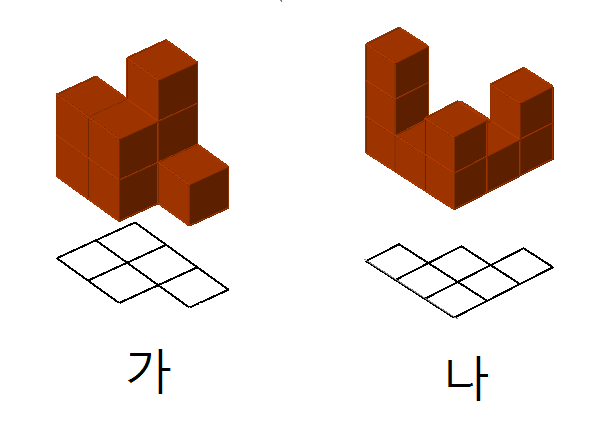
\includegraphics[width=0.7\textwidth]{01-2}
\end{figure}
\par\ans

\prob
똑같은 모양을 만들기 위해 필요한 쌓기나무의 수가 더 적은 것은 어느 것입니까?

\begin{figure}[h]
\centering
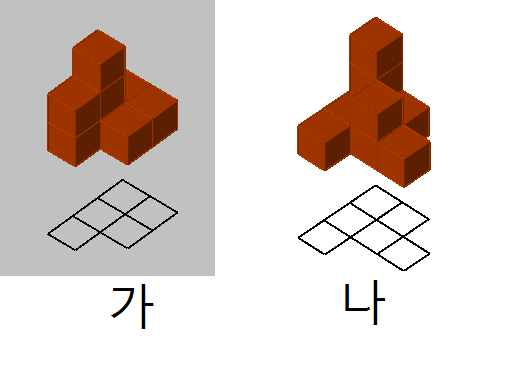
\includegraphics[width=0.7\textwidth]{02}
\end{figure}
\par\ans

\newpage

\prob
쌓기나무로 쌓은 모양을 위, 앞, 옆에서 본 그림입니다.
쌓은 쌓기나무가 가장 적은 경우와 가장 많은 경우는 각각 몇 개 입니까?
\begin{figure}[h]
\centering
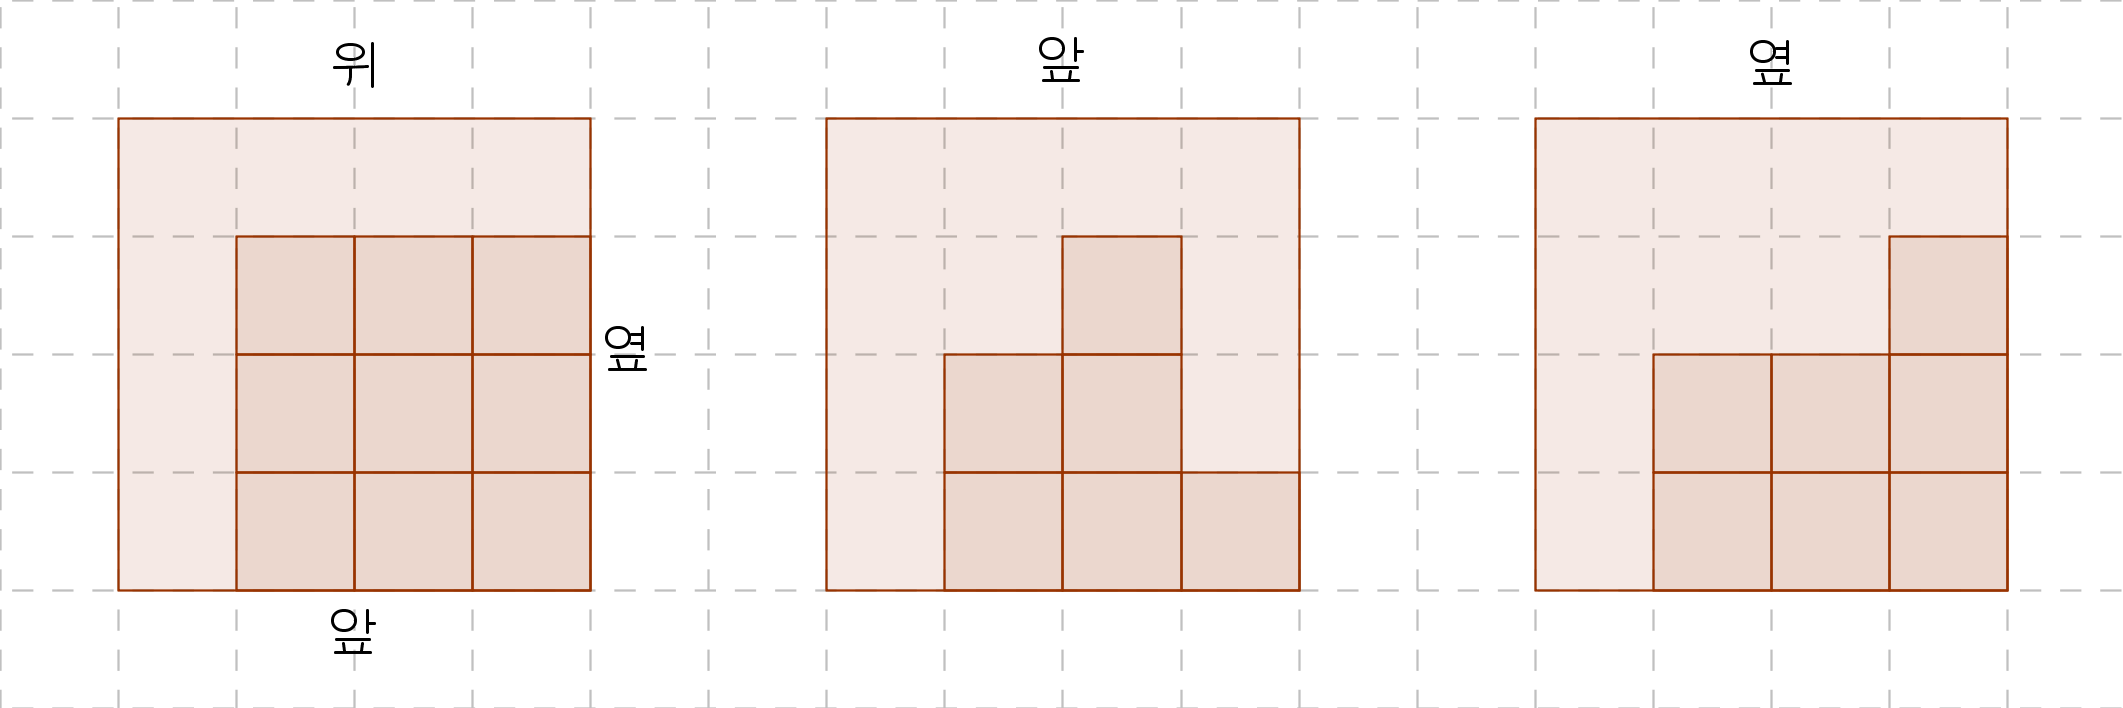
\includegraphics[width=\textwidth]{03}
\end{figure}
{\par\raggedleft\textbf{
가장 적은 경우 : (\qquad\qquad)개\\
가장 많은 경우 : (\qquad\qquad)개}
\par}

\prob
쌓기나무로 쌓은 모양을 위, 앞, 옆에서 본 그림입니다.
쌓은 쌓기나무가 가장 적은 경우와 가장 많은 경우는 각각 몇 개 입니까?
\begin{figure}[h]
\centering
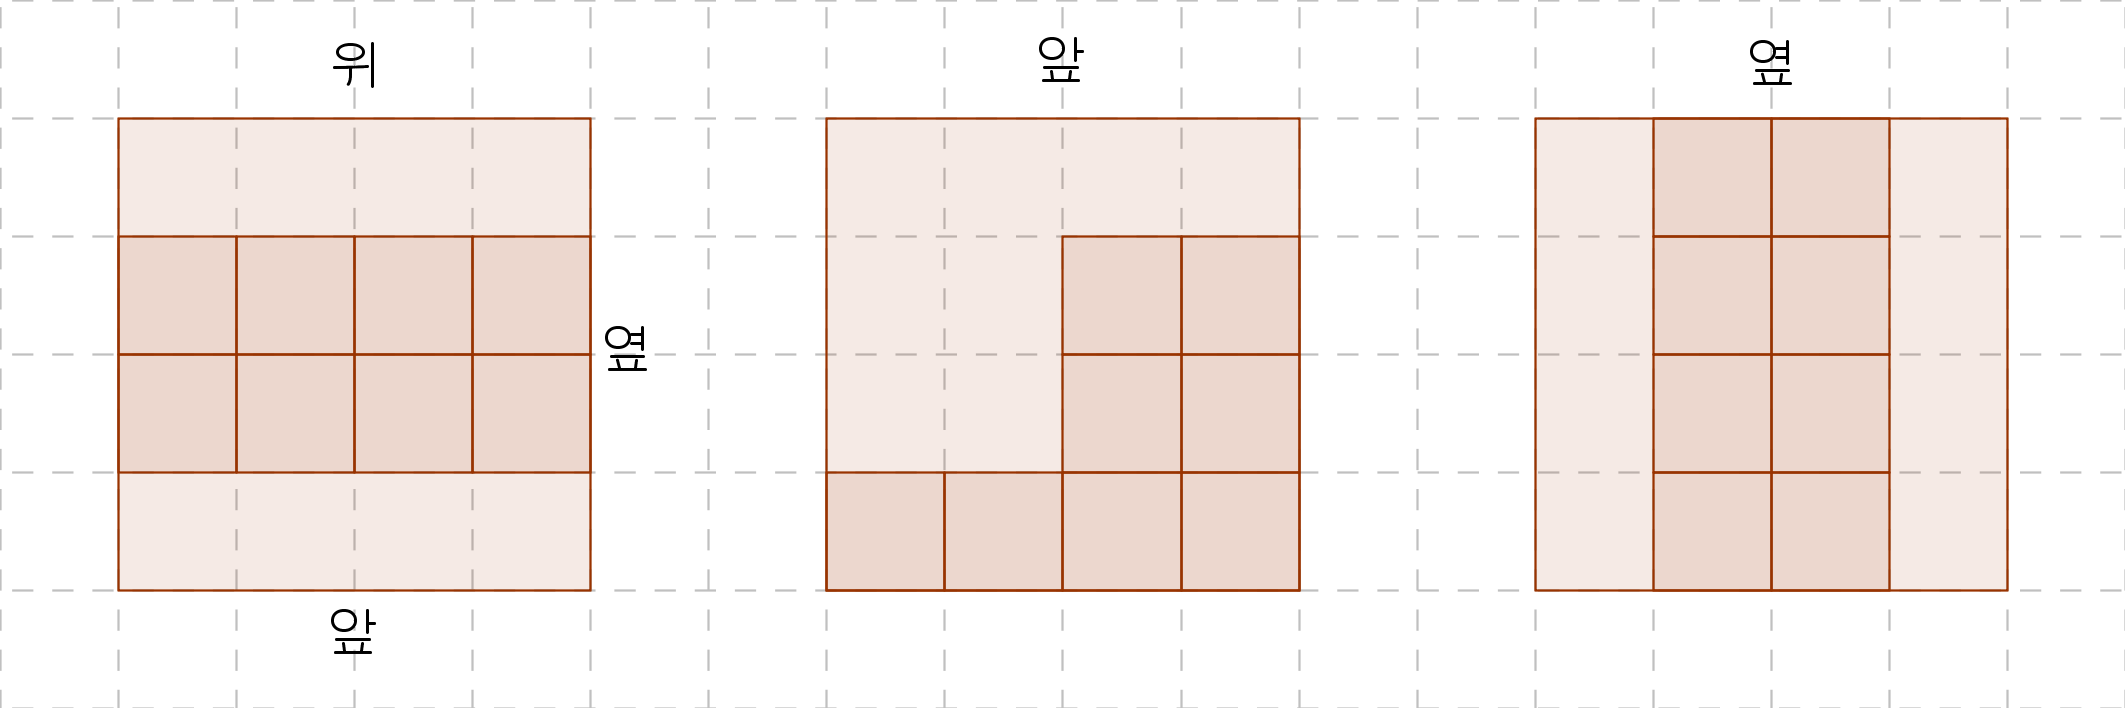
\includegraphics[width=\textwidth]{04}
\end{figure}
{\par\raggedleft\textbf{
가장 적은 경우 : (\qquad\qquad)개\\
가장 많은 경우 : (\qquad\qquad)개}
\par}

\newpage

\prob
쌓기나무로 쌓은 모양을 위, 앞, 옆에서 본 그림입니다.
쌓은 쌓기나무가 가장 적은 경우와 가장 많은 경우의 차는 몇 개 입니까?
\begin{figure}[h]
\centering
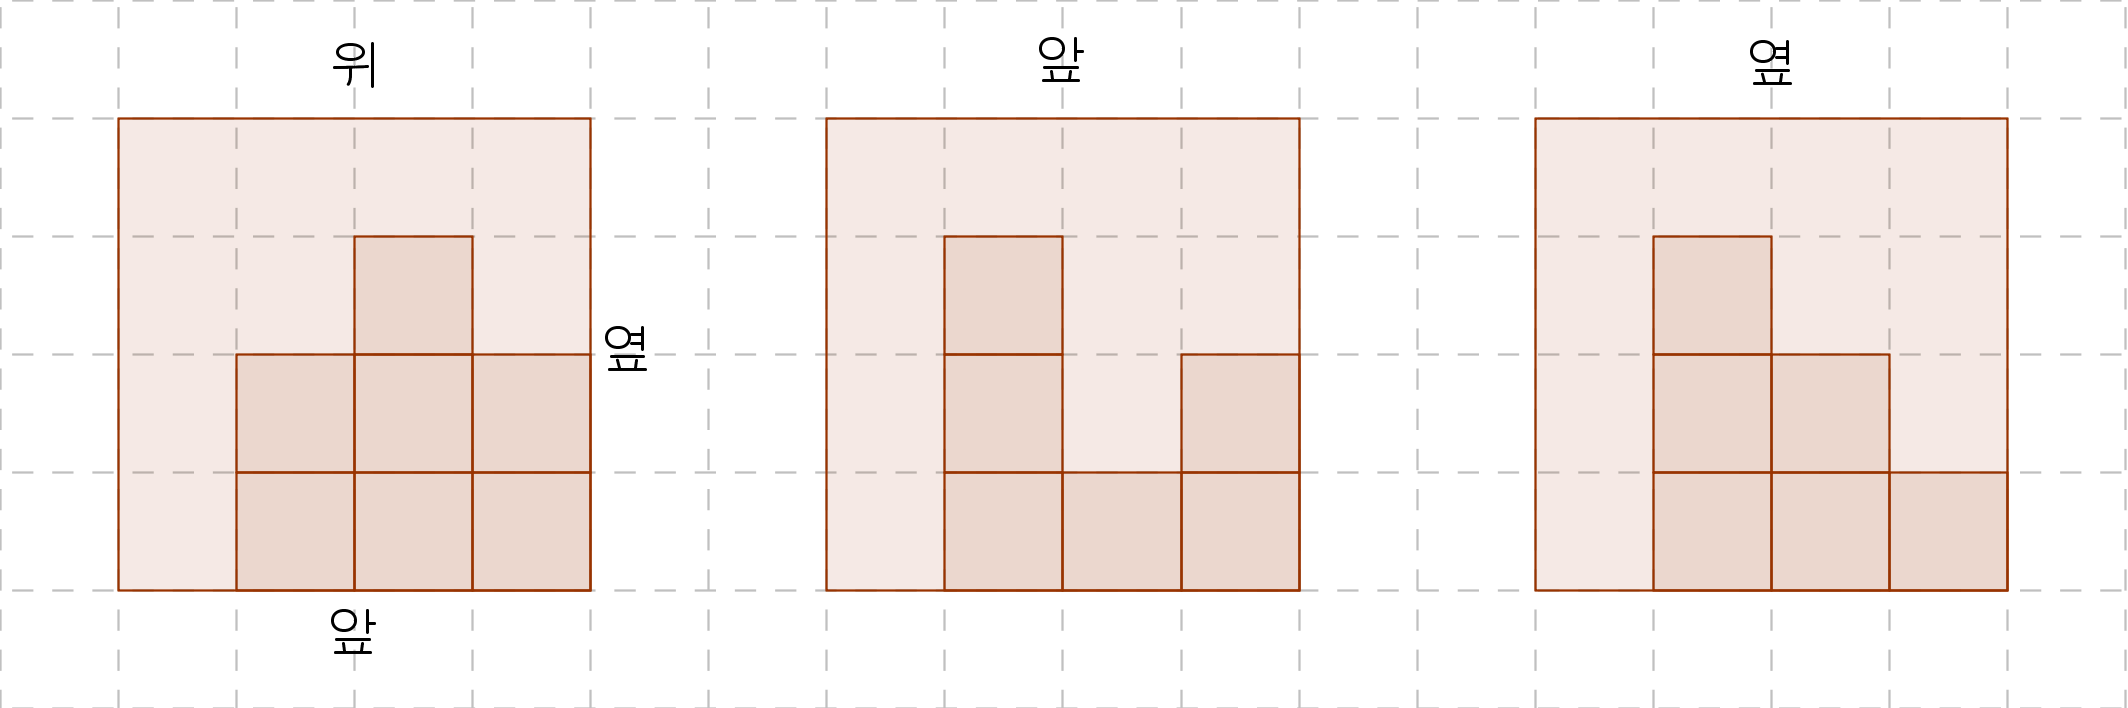
\includegraphics[width=\textwidth]{05}
\end{figure}
{\par\raggedleft\textbf{
가장 적은 경우 : (\qquad\qquad)개\\
가장 많은 경우 : (\qquad\qquad)개\\
차 : (\qquad\qquad)개}
\par}

\prob
쌓기나무로 쌓은 모양을 위, 앞, 옆에서 본 그림입니다.
쌓은 쌓기나무가 가장 적은 경우와 가장 많은 경우의 차는 몇 개 입니까?
\begin{figure}[h]
\centering
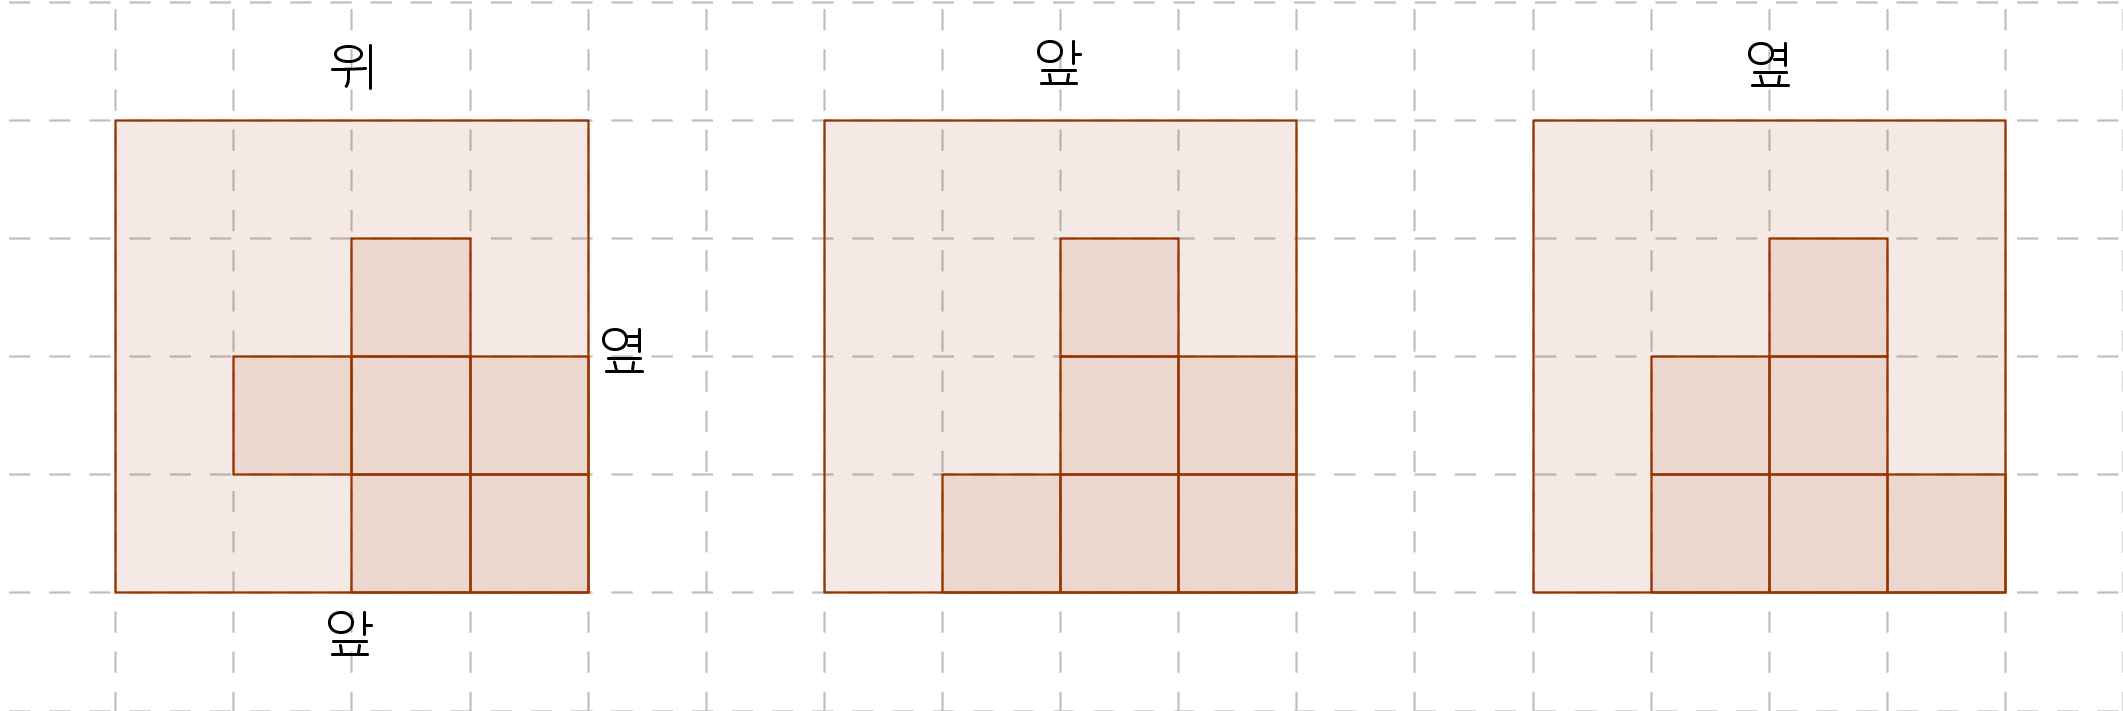
\includegraphics[width=\textwidth]{06}
\end{figure}
{\par\raggedleft\textbf{
가장 적은 경우 : (\qquad\qquad)개\\
가장 많은 경우 : (\qquad\qquad)개\\
차 : (\qquad\qquad)개}
\par}

\newpage

\prob
쌓기나무로 쌓은 모양을 위, 앞, 옆에서 본 그림입니다.
쌓은 쌓기나무가 가장 적은 경우와 가장 많은 경우의 합은 몇 개 입니까?
\begin{figure}[h]
\centering
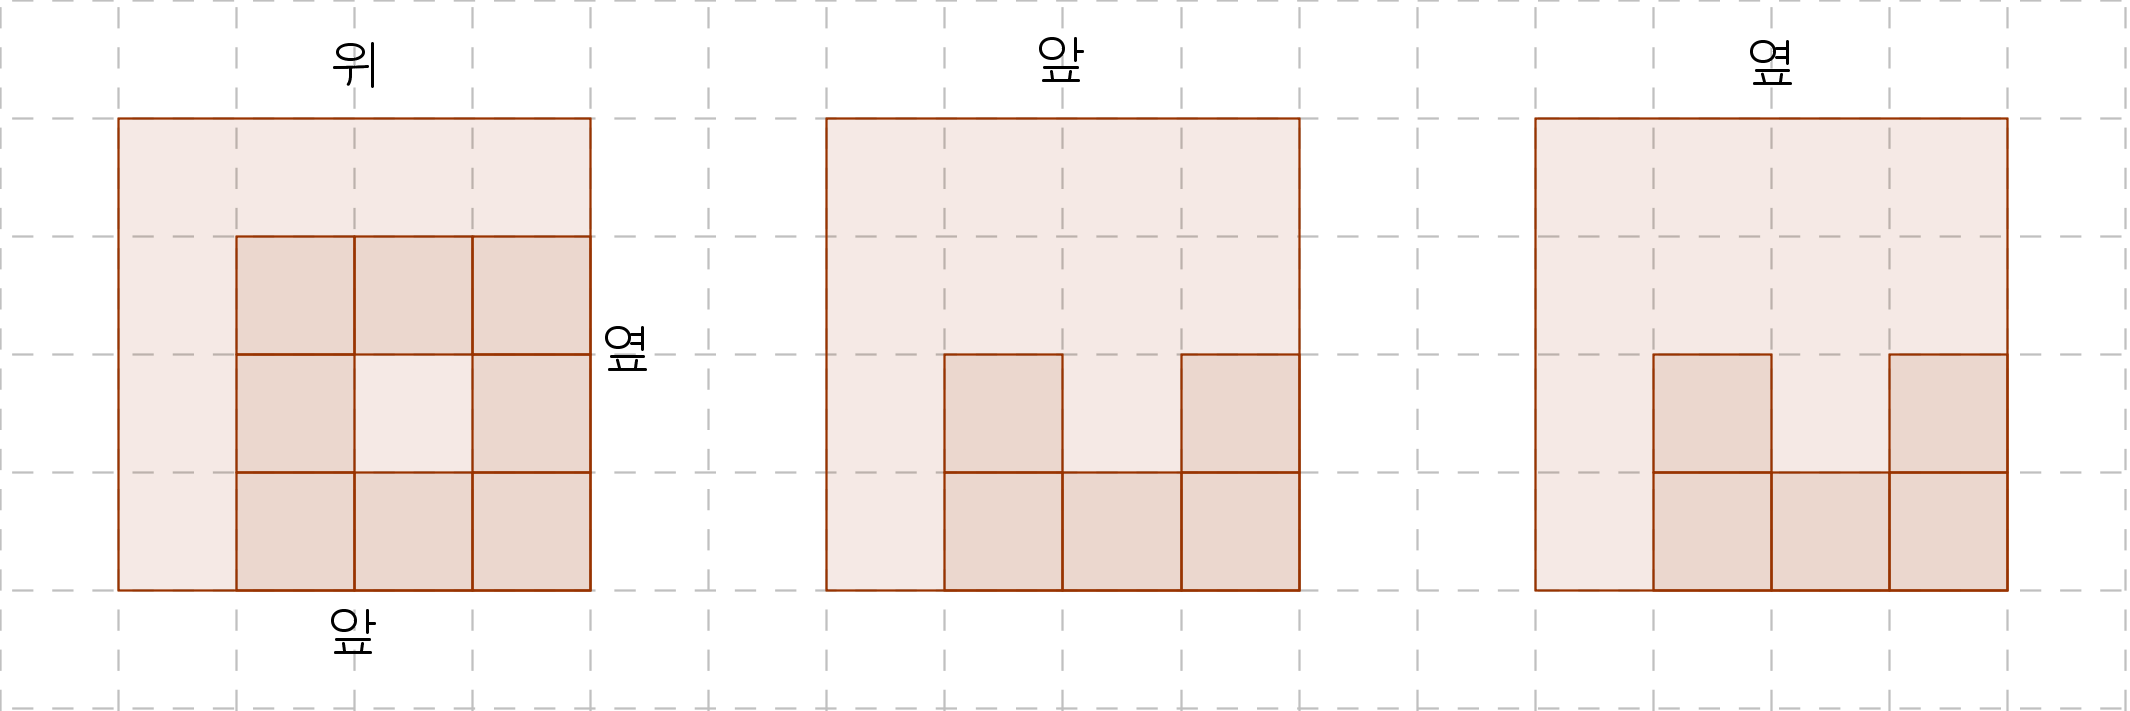
\includegraphics[width=\textwidth]{07}
\end{figure}
{\par\raggedleft\textbf{
가장 적은 경우 : (\qquad\qquad)개\\
가장 많은 경우 : (\qquad\qquad)개\\
합 : (\qquad\qquad)개}
\par}

\prob
쌓기나무로 쌓은 모양을 위, 앞, 옆에서 본 그림입니다.
쌓은 쌓기나무가 가장 적은 경우와 가장 많은 경우의 합은 몇 개 입니까?
\begin{figure}[h]
\centering
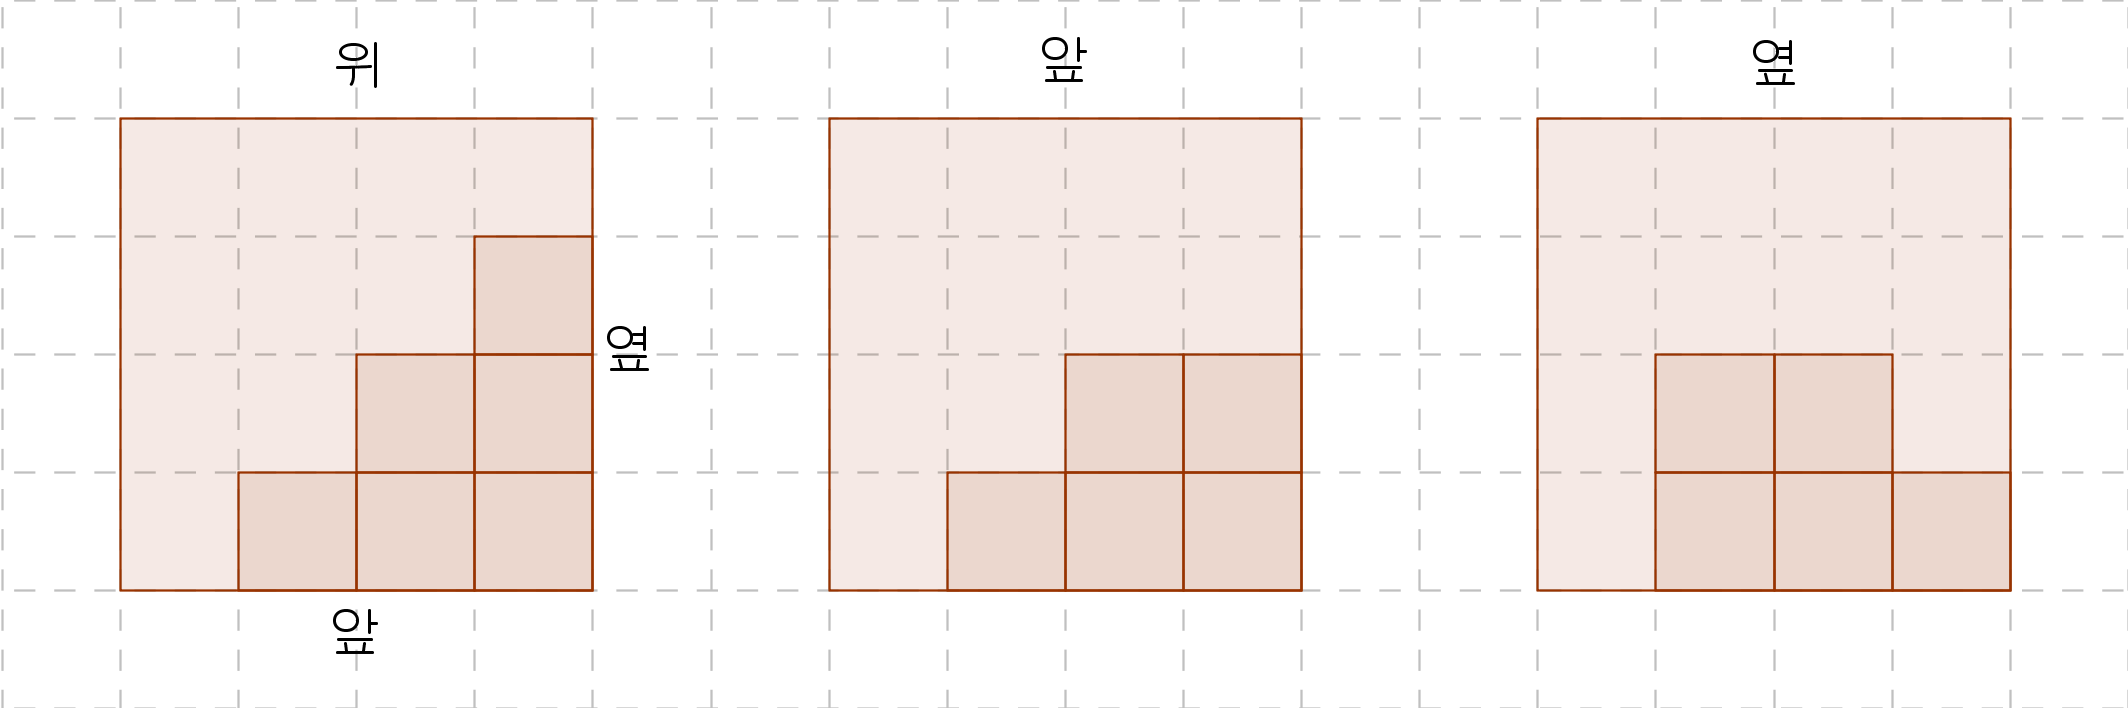
\includegraphics[width=\textwidth]{08}
\end{figure}
{\par\raggedleft\textbf{
가장 적은 경우 : (\qquad\qquad)개\\
가장 많은 경우 : (\qquad\qquad)개\\
합 : (\qquad\qquad)개}
\par}

\prob
아래 그림은 한 변이 1cm인 쌓기나무로 쌓은 모양입니다.
쌓은 모양의 겉넓이는 몇 cm\(^2\)입니까?
\begin{figure}[h]
\centering
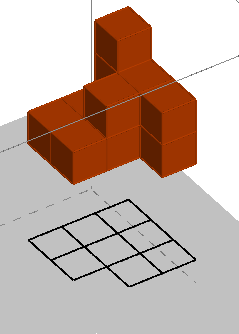
\includegraphics[width=0.35\textwidth]{09}
\end{figure}
{\par\raggedleft\textbf{
답 : (\qquad\qquad\qquad\qquad\qquad)cm\(^2\)}
\par}

\prob
아래 그림은 한 변이 1cm인 쌓기나무로 쌓은 모양입니다.
쌓은 모양의 겉넓이는 몇 cm\(^2\)입니까?
\begin{figure}[h]
\centering
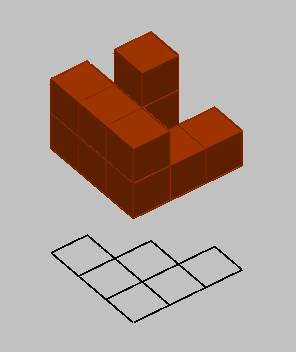
\includegraphics[width=0.35\textwidth]{10}
\end{figure}
{\par\raggedleft\textbf{
답 : (\qquad\qquad\qquad\qquad\qquad)cm\(^2\)}
\par}

\newpage
(돌렸을 때 같은 모양은 한 가지로 생각합니다.)

\prob
쌓기나무 7개를 이용하여 조건을 만족하는 모양은 모두 몇 가지 만들 수 있습니까? 

(1) 쌓기나무로 쌓은 모양은 3층입니다.

(2) 각 층에 놓인 쌓기나무의 개수는 모두 다릅니다.

(3) 위에서 본 그림은 아래 그림과 같습니다.

\begin{figure}[h]
\centering
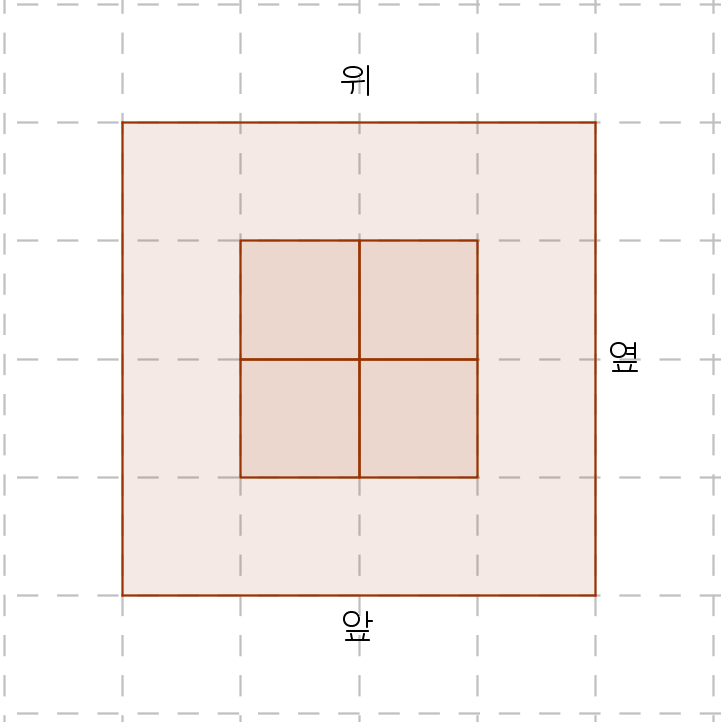
\includegraphics[width=0.35\textwidth]{11}
\end{figure}

\prob
쌓기나무 7개를 이용하여 조건을 만족하는 모양은 모두 몇 가지 만들 수 있습니까? 

(1) 쌓기나무로 쌓은 모양은 3층입니다.

(2) 각 층에 놓인 쌓기나무의 개수는 모두 다릅니다.

(3) 위에서 본 그림은 아래 그림과 같습니다.

\begin{figure}[h]
\centering
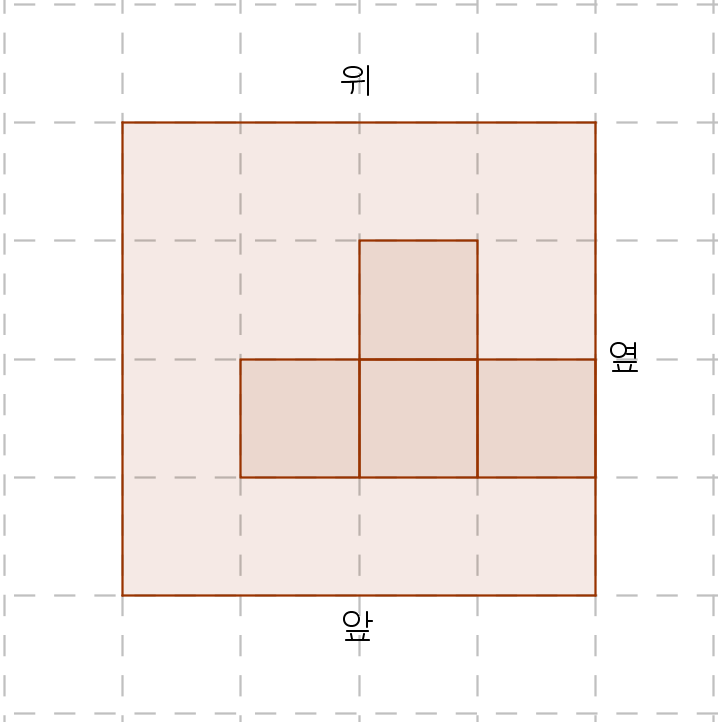
\includegraphics[width=0.35\textwidth]{12}
\end{figure}

\prob
쌓기나무 7개를 이용하여 조건을 만족하는 모양은 모두 몇 가지 만들 수 있습니까? 

(1) 쌓기나무로 쌓은 모양은 3층입니다.

(2) 각 층에 놓인 쌓기나무의 개수는 모두 다릅니다.

(3) 위에서 본 그림은 아래 그림과 같습니다.

\begin{figure}[h]
\centering
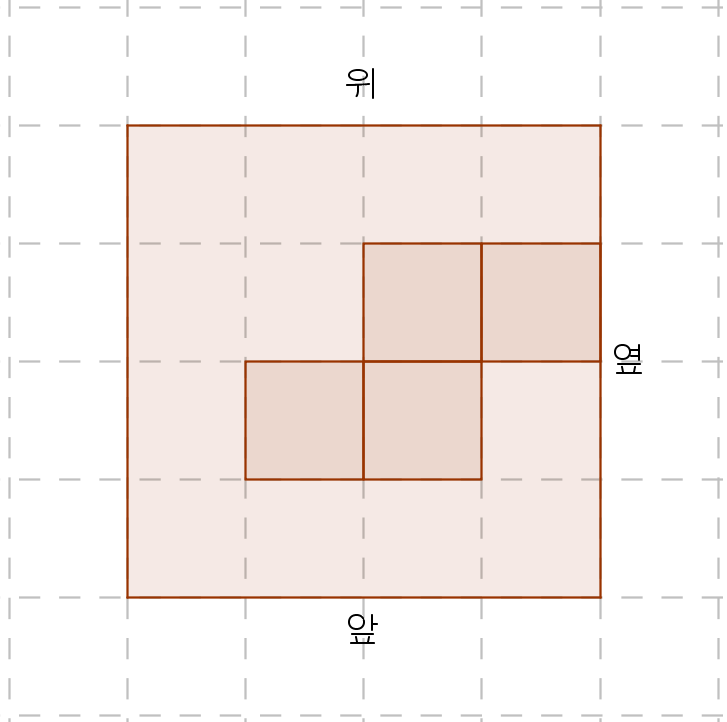
\includegraphics[width=0.35\textwidth]{13}
\end{figure}

\prob
쌓기나무 7개를 이용하여 조건을 만족하는 모양은 모두 몇 가지 만들 수 있습니까? 

(1) 쌓기나무로 쌓은 모양은 3층입니다.

(2) 각 층에 놓인 쌓기나무의 개수는 모두 다릅니다.

(3) 위에서 본 그림은 아래 그림과 같습니다.

\begin{figure}[h]
\centering
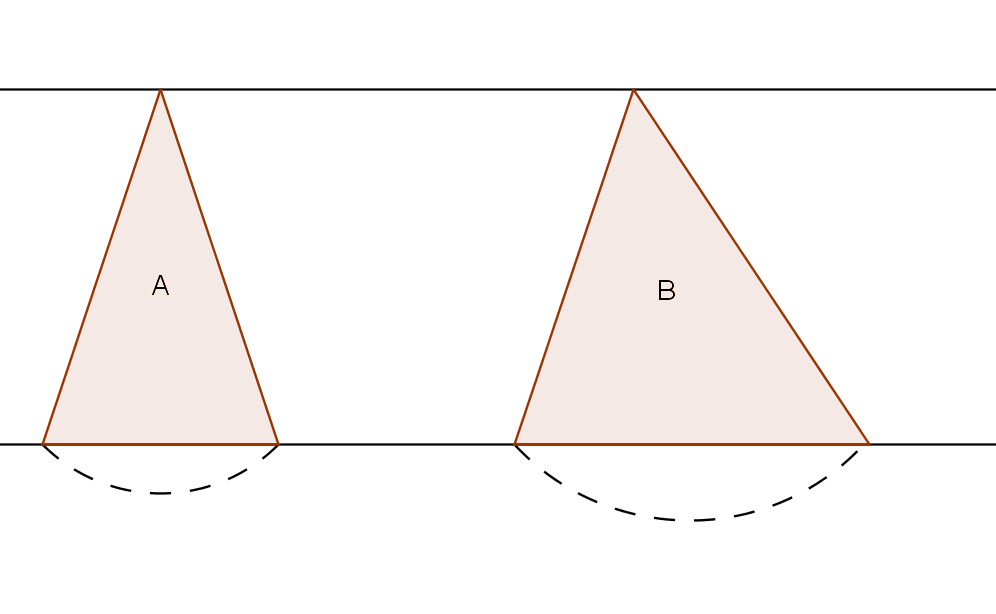
\includegraphics[width=0.35\textwidth]{14}
\end{figure}

\end{document}